\documentclass{article}
% translate with >> pdflatex -shell-escape <file>

\usepackage{pgfplots}
\pgfplotsset{compat=newest}

\pagestyle{empty}

\begin{document}
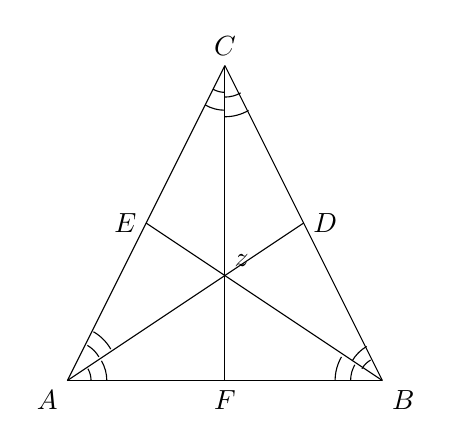
\begin{tikzpicture}%
    \draw (-2, 0) -- (2, 0) (-2, 0) node[anchor = north east] {$A$};
    \draw (2, 0) -- (0, 4) (2, 0) node[anchor = north west] {$B$};
    \draw (-2, 0) -- (0, 4) (0, 4) node[anchor = south] {$C$};
    \draw (2, 0) -- (-1, 2) (-1, 2) node[anchor = east] {$E$};
    \draw (0, 4) -- (0, 0) (0, 0) node[anchor = north] {$F$};
    \draw (-2, 0) -- (1, 2) (1, 2) node[anchor = west] {$D$};
    \draw (0, 1.33) node[anchor= south west] {$z$};
    \draw (-1.7, 0) arc(0:30:3mm);
    \draw (-1.5, 0) arc(0:30:5mm);
    \draw (-1.6, .3) arc(30:60:4mm);
    \draw (-1.45, .4) arc(30:60:6mm);
    \draw (1.85, .26) arc(120:150:3mm);
    \draw (1.8, .433) arc(120:150:5mm);
    \draw (1.65, .2) arc(150:180:4mm);
    \draw (1.48, .3) arc(150:180:6mm);
    \draw (-.15, 3.7) arc(240:270:3mm);
    \draw (-.25, 3.5) arc(240:270:5mm);
    \draw (0, 3.6) arc(270:300:4mm);
    \draw (0, 3.35) arc(270:300:6mm);
\end{tikzpicture}%
\end{document}

